\chapter{Results}

This chapter presents and analyzes the results obtained using the methodology
presented in the previous chapter.

\section{Performance Results}

%The results from using software only for hashing can be seen in table \ref{tab:Perf-SW}.
%The table shows the hashes per second for each active processor as number of processors are scaled up, beginning from Processor 0.
%The different rows are also grouped together, to highlight the distribution.
%The system reaches highest performance with only 3 active processors, and is saturated beyond this point.
%When using additional processors beyond this point, the hashing performance of each processor drops for each new that is added to the system.
%We believe that the stable number on the sum of hashes suggests that access to memory is the main bottleneck.

%It is interesting to note that performance drop for each processor on rows 0-2 no longer drops when fourth row has its processors added, one by one.
%It can also be observed that processor 10 has much greater performance.
%This is likely due to the SHMAC layout, combined with the current XY-routing.
%\todo{Should be improved by numbering the T-tiles in the figure, and cut down this sentence}Processor 10 is the T-tile on 2nd row, to the right edge, seen in figure \ref{fig:5x4}
%With XY-routing, there is no competition for routing between it and the DRAM-tile.
%There is either no competition for routing between the bottom row and the rest of the tiles either.
%This suggests that the mapping on SHMAC can improve or hamper performance, depending on the setup.
%Nevertheless, with memory as main bottleneck, a better mapping will have little effect on performance.
 
Using software-only hashing produced the results in table \ref{tab:Perf-SW}. As can be seen
in the plot in figure \ref{fig:sw-scaling} adding more processors after the third produces no
additional performance gain. \todo{We'll rotate this table or maybe move it to an appendix?}
\todo{Agreed. Marked for future fix}
The reason for this is that all cores must make frequent accesses to DRAM, which causes the
DRAM tile to quickly become congested.

Another interesting effect to note in the results is how the XY routing affects the performance
of each tile. The more tiles that tries to access main memory through a tile, the less
performance that tile has; it seems that SHMACs router system favours requests originating
from other tiles before requests originating from the tile itself.

Exceptions are processor tile 10, which appears to have no competition with other tiles for the routing, and row 4, as adding processors from this row seems does not decrease the individual performance of other tiles. 

\begin{flushleft}
\begin{table}
\tiny
\begin{tabular}{| l || r r r r | r r r r | r r r | r r r r r |}
  \hline 
  \textbf{Sum} [H/s] & \textbf{0} & \textbf{1} & \textbf{2} & \textbf{3} & \textbf{4} & \textbf{5} & \textbf{6} & \textbf{7} & \textbf{8} & \textbf{9} & \textbf{10} & \textbf{11} & \textbf{12} & \textbf{13} & \textbf{14} & \textbf{15}   \\
  \hline                       
  \textbf{13041} & 13041 & - & - & - & - & - & - & - & - & - & - & - & - & - & - & - \\
  \textbf{26105} & 13041 & 13064 & - & - & - & - & - & - & - & - & - & - & - & - & - & - \\
  \textbf{39185} & 13041 & 13064 & 13080 & - & - & - & - & - & - & - & - & - & - & - & - & - \\
  \textbf{36470} & 11114 & 10801 & 7258 & 7297 & - & - & - & - & - & - & - & - & - & - & - & - \\
  \textbf{36449} & 8064 & 8033 & 4065 & 4063 & 12224 & - & - & - & - & - & - & - & - & - & - & - \\
  \textbf{36452} & 6063 & 6073 & 3047 & 3047 & 9140 & 9082 & - & - & - & - & - & - & - & - & - & - \\
  \textbf{36450} & 4237 & 4244 & 2125 & 2125 & 6367 & 6367 & 10985 & - & - & - & - & - & - & - & -\\
  \textbf{36457} & 4044 & 4051 & 2027 & 2027 & 6077 & 6077 & 6077 & 6077 & - & - & - & - & - & - & - \\
  \textbf{36446} & 2686 & 2691 & 1345 & 1345 & 4035 & 4035 & 4035 & 4035 & 12239 & - & - & - & - & - & - & -\\
  \textbf{36457} & 2022 & 2026 & 1013 & 1013 & 3039 & 3039 & 3039 & 3039 & 9131 & 9096 & - & - & - & - & - & -\\
  \textbf{37640} & 1463 & 1467 & 733 & 733 & 2200 & 2200 & 2200 & 2200 & 6600 & 6600 & 11244 & - & - & - & - & -\\
  \textbf{36442} & 1017 & 1021 & 511 & 511 & 1531 & 1531 & 1531 & 1531 & 4595 & 4595 & 9188 & 8880 & - & - & - & -\\
  \textbf{36868} & 1020 & 1035 & 517 & 517 & 1550 & 1550 & 1550 & 1550 & 4656 & 4656 & 9161 & 4553 & 4553 & - & - & -\\
  \textbf{36447} & 1012 & 1016 & 508 & 508 & 1525 & 1525 & 1525 & 1525 & 4573 & 4573 & 9146 & 2266 & 2266 & 4479 & - & -\\
  \textbf{36444} & 1010 & 1014 & 507 & 507 & 1521 & 1521 & 1521 & 1521 & 4564 & 4564 & 9128 & 1524 & 1524 & 3031 & 2987 & -\\
  \textbf{37645} & 1042 & 1046 & 523 & 523 & 1569 & 1569 & 1569 & 1569 & 4706 & 4706 & 9411 & 1572 & 1572 & 3124 & 1572 & 1572\\
  \hline  
\end{tabular}
\caption{Software hash results, using varying numbers of cores. Distribution on different tile-rows are highlighted by column separation}
\label{tab:Perf-SW}
\end{table}
\end{flushleft}

\begin{figure}
	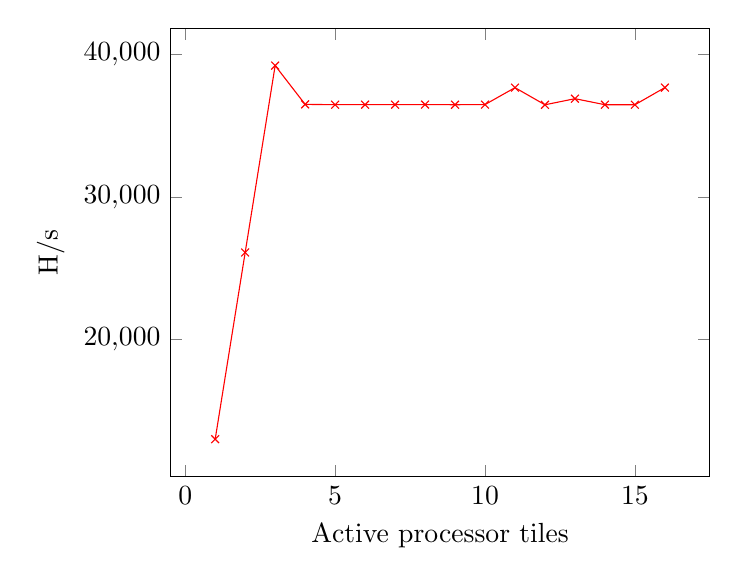
\begin{tikzpicture}
		\begin{axis}[
			xlabel=Active processor tiles,
			ylabel=H/s,
			scaled ticks=false]
		\addplot[color=red,mark=x] coordinates {
			(1, 13041)
			(2, 26105)
			(3, 39185)
			(4, 36470)
			(5, 36449)
			(6, 36452)
			(7, 36450)
			(8, 36457)
			(9, 36446)
			(10, 36457)
			(11, 37640)
			(12, 36442)
			(13, 36868)
			(14, 36447)
			(15, 36444)
			(16, 37645)
		};
		\end{axis}
	\end{tikzpicture}
	\caption{Scaling using software hashing}
	\label{fig:sw-scaling}
\end{figure}

Tables \ref{tab:Perf-SHA} and \ref{tab:Perf-SHADMA} shows the results when using the SHA-256 hashing accelerator, and without and with DMA module, respectively.
Only up to four processors where used, as adding in processors from the second row when scaling from processor 0 caused the application to crash.
The cause is currently unknown.

Both tables shows that the sum of hashes has a near-linear increase, with very low indiviual performance drop.
It appears that the individual perfomance of each processor varies, with some higher than others, and so far they remain stable. 
The application uses scratchpad tiles when the SHA-256 hashing module is in use, and positioning combined with XY-routing may be the reason behind the variying performance.

Using DMA shows the same trend, but with increased performance for each tile.

\begin{table}
\begin{tabular}{| l || r r r r |}
  \hline 
  \textbf{Sum} [H/s] & \textbf{0} & \textbf{1} & \textbf{2} & \textbf{3}\\
  \hline                       
  \textbf{37711} & 37711 & - & - & - \\
  \textbf{80237} & 37655 & 42582 & - & - \\
  \textbf{117791} & 37556 & 42450 & 37785 & - \\
  \textbf{150799} & 37391 & 42271 & 37496 & 33641 \\
  \hline  
\end{tabular}
\caption{Hashing per second, using the SHA256-hashing module. Only up to 4 processors worked}
\label{tab:Perf-SHA}
\end{table}

\begin{table}
\begin{tabular}{| l || r r r r |}
  \hline 
  \textbf{Sum} [H/s] & \textbf{0} & \textbf{1} & \textbf{2} & \textbf{3}\\
  \hline                       
  \textbf{42209} & 42209 & - & - & - \\
  \textbf{86979} & 41787 & 45192 & - & - \\
  \textbf{126705} & 41097 & 44456 & 41152 & - \\
  \textbf{159372} & 39799 & 43303 & 39824 & 36446 \\
  \hline  
\end{tabular}
\caption{Hashing per second, using the SHA256-hashing module and DMA module. Only up to 4 processors worked}
\label{tab:Perf-SHADMA}
\end{table}

The results are compared in \ref{fig:Perf-plot}, where software hashing is seen in red, accelerator hashing is seen in blue, and accelerator hashing using DMA is seen in black.
As seen in the figure, the hashing modules far outperforms the software hashing, even with only up to four processors in use.

\begin{figure}
	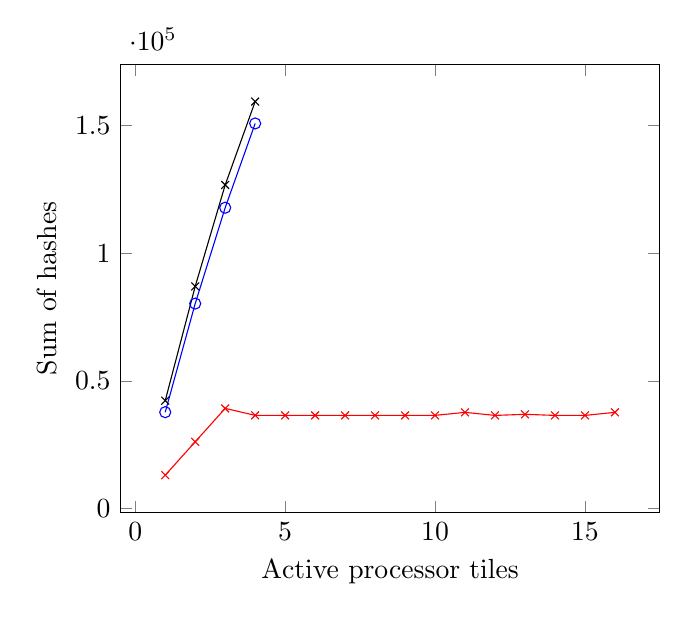
\begin{tikzpicture}
		\begin{axis}[
			xlabel=Active processor tiles,
			ylabel=Sum of hashes]
		\addplot[color=red,mark=x] coordinates {
			(1, 13041)
			(2, 26105)
			(3, 39185)
			(4, 36470)
			(5, 36449)
			(6, 36452)
			(7, 36450)
			(8, 36457)
			(9, 36446)
			(10, 36457)
			(11, 37640)
			(12, 36442)
			(13, 36868)
			(14, 36447)
			(15, 36444)
			(16, 37645)
		};
		\addplot[color=blue,mark=o] coordinates {
			(1, 37711)
			(2, 80237)
			(3, 117791)
			(4, 150799)
		};
		\addplot[color=black,mark=x] coordinates {
			(1, 42209)
			(2, 86979)
			(3, 126705)
			(4, 159372)
		};
		\end{axis}
	\end{tikzpicture}
	\caption{Sum of hashes per second. Red: SW only, Blue: SHA-256 only, Black: SHA-256 + DMA}
	\label{fig:Perf-plot}
\end{figure}

\section{Power and energy efficiency}

We must measure the power from the wall, before we can add anything here.












